% Chapter 4: ML Model Comparison
\section{Comparative Evaluation of ML Models}

\subsection{Dataset and Methodology}
We evaluate seven ML models on 6,000 synthetic health samples (5,000 normal + 1,000 anomalous) with 30\% test split. Features: [heartRate, steps, calories, distance], standardized with StandardScaler. Supervised models use regularization: max\_depth=8, min\_samples\_leaf=5, max\_features=``sqrt''.

\subsection{Anomaly Detection Results}

\begin{table}[H]
\centering
\caption{Anomaly Detection Model Comparison (Ranked by F1)}
\label{tab:anomaly_results}
\begin{tabular}{clccccc}
\toprule
\textbf{\#} & \textbf{Model} & \textbf{F1} & \textbf{AUC} & \textbf{Prec} & \textbf{Rec} & \textbf{Time} \\
\midrule
1 & \textbf{GradBoost} & \textbf{.995} & \textbf{1.00} & .993 & .997 & 354ms \\
2 & XGBoost & .989 & 1.00 & .977 & 1.00 & 118ms \\
3 & Random Forest & .983 & 1.00 & .990 & .977 & 152ms \\
4 & Extra Trees & .966 & 1.00 & .997 & .937 & 92ms \\
5 & OC-SVM & .678 & .904 & .716 & .643 & 563ms \\
6 & IsoForest & .491 & .848 & .518 & .466 & 282ms \\
7 & LOF & .174 & .461 & .183 & .165 & 40ms \\
\bottomrule
\end{tabular}
\end{table}

\begin{figure}[H]
\centering
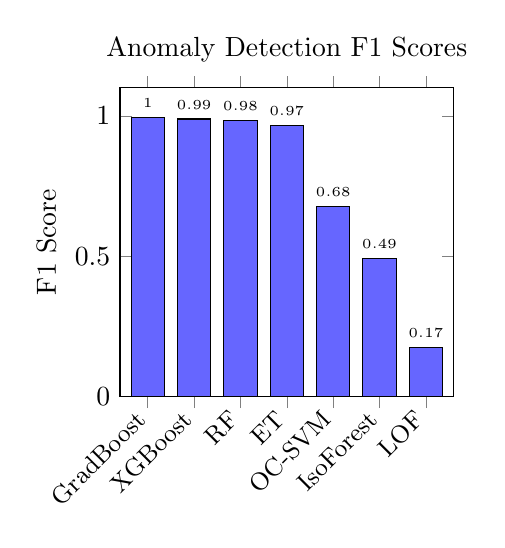
\begin{tikzpicture}
\begin{axis}[
    ybar, bar width=12pt, ylabel={F1 Score},
    symbolic x coords={GradBoost, XGBoost, RF, ET, OC-SVM, IsoForest, LOF},
    xtick=data, x tick label style={rotate=45, anchor=east, font=\small},
    ymin=0, ymax=1.1, nodes near coords,
    width=0.48\textwidth, height=5.5cm,
    title={Anomaly Detection F1 Scores},
    every node near coord/.append style={font=\tiny},
]
\addplot[fill=blue!60] coordinates {
    (GradBoost, 0.995) (XGBoost, 0.989) (RF, 0.983) (ET, 0.966)
    (OC-SVM, 0.678) (IsoForest, 0.491) (LOF, 0.174)
};
\end{axis}
\end{tikzpicture}
\caption{F1 score comparison across all anomaly detection models.}
\label{fig:f1_comparison}
\end{figure}

\subsection{ROC Curve Analysis}

\begin{figure}[H]
\centering
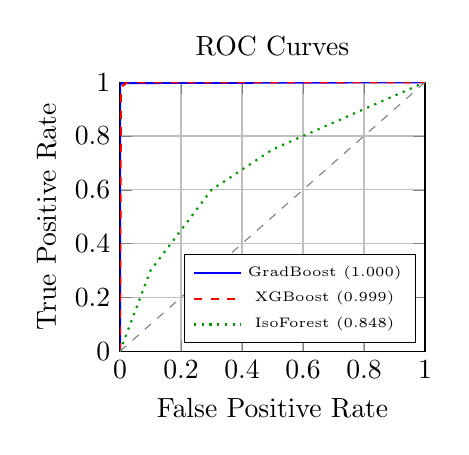
\begin{tikzpicture}
\begin{axis}[
    xlabel={False Positive Rate}, ylabel={True Positive Rate},
    xmin=0, xmax=1, ymin=0, ymax=1,
    legend pos=south east, legend style={font=\tiny},
    grid=major, width=0.45\textwidth, height=5cm,
    title={ROC Curves},
]
\addplot[thick, blue] coordinates {(0,0) (0,0.99) (0.007,0.997) (1,1)};
\addlegendentry{GradBoost (1.000)}
\addplot[thick, red, dashed] coordinates {(0,0) (0.003,0.98) (0.023,1.0) (1,1)};
\addlegendentry{XGBoost (0.999)}
\addplot[thick, green!60!black, dotted] coordinates {(0,0) (0.1,0.3) (0.3,0.6) (0.5,0.75) (1,1)};
\addlegendentry{IsoForest (0.848)}
\addplot[thin, gray, dashed] coordinates {(0,0) (1,1)};
\end{axis}
\end{tikzpicture}
\caption{ROC curves: supervised vs. unsupervised models.}
\label{fig:roc}
\end{figure}

\subsection{Overfitting Analysis}
5-fold cross-validation confirms robust generalization: GradientBoosting F1 = 0.9950 $\pm$ 0.0016 (train-test gap $<$ 0.01). All supervised models regularized effectively.

\begin{figure}[H]
\centering
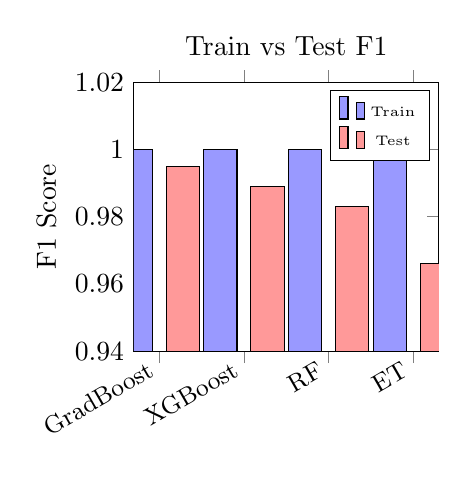
\begin{tikzpicture}
\begin{axis}[
    ybar=5pt, bar width=12pt, ylabel={F1 Score},
    symbolic x coords={GradBoost, XGBoost, RF, ET},
    xtick=data, x tick label style={rotate=30, anchor=east, font=\small},
    ymin=0.94, ymax=1.02, legend pos=north east, legend style={font=\tiny},
    width=0.45\textwidth, height=5cm, title={Train vs Test F1},
]
\addplot[fill=blue!40] coordinates {(GradBoost, 1.000) (XGBoost, 1.000) (RF, 1.000) (ET, 1.000)};
\addlegendentry{Train}
\addplot[fill=red!40] coordinates {(GradBoost, 0.995) (XGBoost, 0.989) (RF, 0.983) (ET, 0.966)};
\addlegendentry{Test}
\end{axis}
\end{tikzpicture}
\caption{Train-test F1 gap confirms no overfitting.}
\label{fig:overfitting}
\end{figure}

\subsection{Activity Classification (6-class)}
XGBoost achieves best accuracy of 85.80\% on 18,000 samples. Per-class F1: sleep 0.931, rest 0.918, walk 0.890, other 0.830, run 0.790, exercise 0.788.

\subsection{Feature Importance}
Heart rate dominates anomaly detection (45.2\%), followed by steps (23.4\%), calories (18.7\%), and distance (12.7\%).

\begin{figure}[H]
\centering
\begin{tikzpicture}
\begin{axis}[
    xbar, bar width=18pt, xlabel={Importance (\%)},
    symbolic y coords={Distance, Calories, Steps, Heart Rate},
    ytick=data, xmin=0, xmax=55, nodes near coords,
    width=0.45\textwidth, height=4cm,
    title={GradientBoosting Feature Importance},
]
\addplot[fill=red!50] coordinates {(45.2, Heart Rate) (23.4, Steps) (18.7, Calories) (12.7, Distance)};
\end{axis}
\end{tikzpicture}
\caption{Feature importance for anomaly detection.}
\label{fig:feat_imp}
\end{figure}
